\section{Data}
\label{sec:data}
\emph{In short: the record, the common preselection ($23{,}895$ candidates) and the fit window ($19{,}731$ candidates); the spectrum peaks at $5284\,\MeV$ for both charges and both polarities, and the counting asymmetry is $-0.043\pm0.007$.}
\subsection{Dataset, Preselection and Mass}
\label{sec:data_presel}
The dataset is the CERN Open Data record 4900~\cite{opendata_record}: $B^{\pm}\to h^{\pm}h^{+}h^{-}$ candidates collected by LHCb in 2011 at $\sqrt{s}=7$\,TeV, already through trigger and offline selection, split by magnet polarity ($8{,}556{,}118$ candidates), and a detector-free phase-space simulation of $B^{\pm}\to K^{\pm}K^{+}K^{-}$ ($50{,}000$ decays, no asymmetry) used only to test the local-asymmetry procedure (Sec.~\ref{sec:dalitz}). The same preselection is used in all analyses,
\[
\texttt{H*\_ProbPi} < 0.5 \ \wedge\ \texttt{H*\_ProbK} > 0.5 \ \wedge\ \lnot\texttt{H*\_isMuon},
\]
for each of the three tracks, and retains $23{,}895$ candidates ($0.28\%$). $H1$ is always the kaon of charge opposite to the $B$ and $H2$, $H3$ are the same-sign pair, so the Dalitz variables are the two opposite-sign invariant masses $m^2(H1,H2)$ and $m^2(H1,H3)$.
\label{sec:data_mass}
The three tracks are assigned the charged-kaon mass and their four-momenta are summed to reconstruct $m(KKK)$. The \textbf{nominal fit window}, common to the two analyses, is $[5100,5600]\,\MeV$ and contains $19{,}731$ candidates ($11{,}636$ magnet down, $8095$ magnet up). Below $\sim$5150\,\MeV\ the background rises, which a single exponential cannot describe; the window includes the start of this rise, described by a second exponential in the background model (Secs.~\ref{sec:frequentist}--\ref{sec:bayesian}).
\subsection{Data Exploration}
\label{sec:data_exploration}

Figure~\ref{fig:mass_spectrum} shows the spectrum in the fit window. The peak at $m\approx5284\,\MeV$ over a falling combinatorial background has the same shape for the two charges and the two polarities, which allows a mass and a resolution common to $B^+$ and $B^-$ in the model (Sec.~\ref{sec:model}). The \emph{counting asymmetry} of all candidates, signal and background together, is $A_{\mathrm{count}}=(N^--N^+)/(N^-+N^+)=-0.043\pm0.007$ (binomial uncertainty); the fits of Secs.~\ref{sec:frequentist} and \ref{sec:bayesian} refine it by separating signal and background.

\begin{figure}[t]
\centering
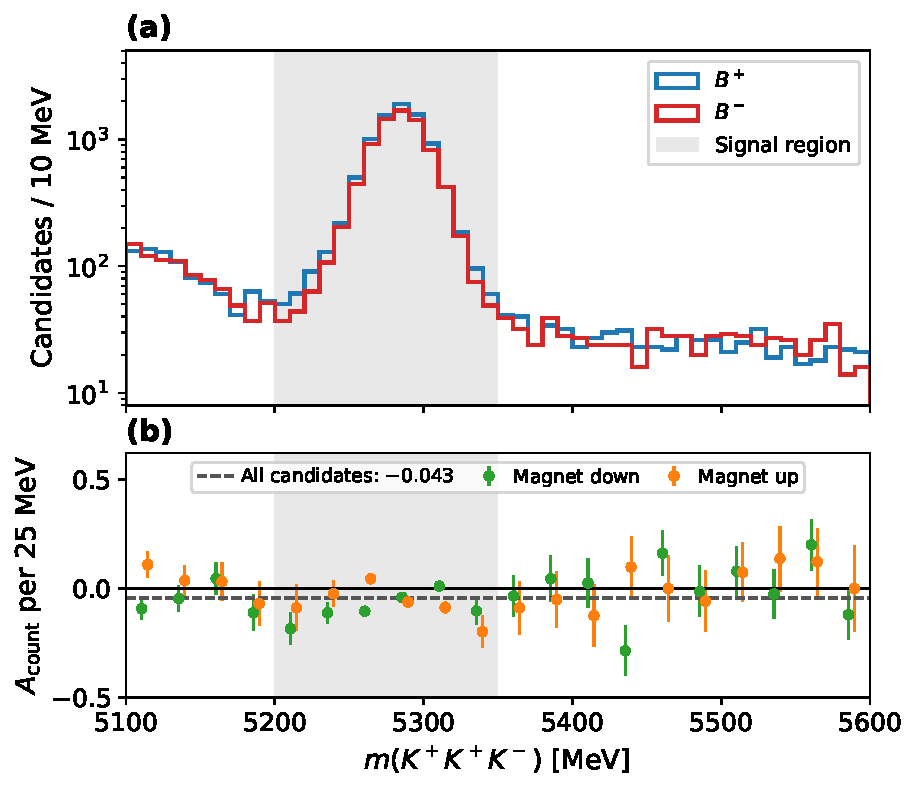
\includegraphics[width=\columnwidth]{figures/mass_spectrum_col.pdf}
\caption{(a) Reconstructed $B\to KKK$ invariant mass in the nominal fit window $[5100,5600]\,\MeV$ for $B^+$ and $B^-$, logarithmic scale; the signal region $[5200,5350]\,\MeV$ is shaded. (b) Counting asymmetry in $25\,\MeV$ bins of the mass for the two magnet polarities, and for all candidates (dashed); the two polarities agree within their uncertainties and the asymmetry is similar in the peak and in the sidebands.}
\label{fig:mass_spectrum}
\end{figure}

\subsection{Additional Results}

\emph{Selection.} The kaon-identification requirement on the three tracks is by far the most selective step of the preselection, and only $42$ candidates of the fit window ($0.2\%$) share a track with another candidate; all are kept.
